\documentclass[11pt]{article}
% ============================================================
% Bibliography backend: biblatex + biber
% ============================================================
\usepackage[backend=biber,style=numeric,sorting=none]{biblatex}
\addbibresource{../shared/references.bib}

\usepackage{amsmath,amssymb}
% --- Graphics / TikZ ---
\usepackage{tikz}
\usetikzlibrary{arrows.meta,calc,decorations.pathreplacing}
% shared/macros.tex
\providecommand{\Afive}{A_{5}}
\providecommand{\golden}{\varphi} % optional standard name for \varphi
\providecommand{\phig}{\varphi}
\providecommand{\dd}{\mathrm{d}}
\providecommand{\ii}{\mathrm{i}}
\providecommand{\ee}{\mathrm{e}}
\providecommand{\Tr}{\mathrm{Tr}}
\providecommand{\diag}{\mathrm{diag}}
\providecommand{\SU}{\mathrm{SU}}
\providecommand{\U}{\mathrm{U}}


% ============================================================
% GPP_DRAFT_SUPPRESS_WARNINGS
% Draft-mode suppression of undefined reference warnings.
% Toggle: set \GPPdrafttrue (on) / \GPPdraftfalse (off)
% ============================================================
\newif\ifGPPdraft
\GPPdrafttrue

\makeatletter
\ifGPPdraft
  % Suppress only warning emissions (keeps errors, overfull boxes, etc.)
  \def\@latex@warning@no@line#1{}
  \def\@latex@warning#1{}
\fi
\makeatother



\title{Golden Unification: Collected Drafts}
\author{}
\date{}

\begin{document}
\maketitle

\clearpage
\section*{Paper I}
% ============================================================
% Auto-generated canonical body file for Paper I
% DO NOT place content here directly.
% Edit section files under papers/sections/
% ============================================================

\section{Discrete Logarithmic Structure in Flavor Data}
\label{sec:log_structure}

Fermion masses in the Standard Model span more than twelve orders of magnitude, from
sub-eV neutrino scales to the top-quark mass near the electroweak scale. When represented
on linear axes, this hierarchy appears irregular and weakly structured. However, when
expressed in logarithmic coordinates, mass ratios become additive quantities, and potential
organizational regularities---if present---are rendered more transparent.

This observation is not new in itself: renormalization-group flow, dimensional transmutation,
and hierarchical symmetry breaking naturally generate exponential relations among physical
scales. What is less commonly emphasized is that, when logarithmic mass ratios are compared
directly across particle species under fixed conventions, the observed spectrum can exhibit
non-random clustering suggestive of discrete organization.

In this work we therefore adopt logarithmic coordinates as the natural arena in which to
examine structural regularities in flavor data. Writing each mass as
\begin{equation}
m_i \;=\; m_{\mathrm{ref}} \, e^{\Delta_i},
\end{equation}
the dimensionless quantities $\Delta_i$ encode relative mass information independently of
the choice of reference scale $m_{\mathrm{ref}}$. Throughout, all comparisons are performed
in such dimensionless logarithmic variables.

The central empirical hypothesis explored here is that measured fermion masses and associated
flavor observables cluster near a discrete subset of logarithmic values once a reference
convention is fixed. In the construction used in this paper, the relevant discreteness is
expressed in base-$\varphi$ logarithms with quarter-integer spacing (with half-integer and
integer steps appearing as special cases; see Sec.~\ref{sec:lattice}). Importantly, this
hypothesis does not posit a mass-generation mechanism, an underlying symmetry, or a dynamical
explanation. Rather, it asserts only the existence---or absence---of a reproducible regularity
in the data under explicitly declared constructions.

Our objective is therefore deliberately limited. We do not assume that the observed structure
reflects a fundamental law, nor do we infer ultraviolet dynamics from it. Instead, we document
the regularity itself using a transparent, auditable framework and specify clear falsification
criteria. In particular, any claimed clustering must persist under controlled perturbations of
input data, anchoring choices, and bounded scan protocols. Failure to do so constitutes evidence
against the organizing principle.

Throughout, the emphasis is on reproducibility, explicit assumptions, and sharply delimited
interpretation. Questions of deeper meaning---if any---are deferred until after the empirical
structure has been established or ruled out.
\section{Logarithmic Lattice and Anchoring Conventions}
\label{sec:lattice}

To test whether fermion masses admit a discrete organization in logarithmic space,
we must specify both the coordinate representation in which comparisons are made
and a fixed convention that removes trivial global rescalings. This section defines
the anchored lattice construction used throughout the paper. The construction is
methodological rather than interpretive: once fixed, it is held constant across all
analyses reported here.

\subsection{Logarithmic coordinates and reference normalization}

Given a set of measured masses $\{m_i\}$ and a reference mass $m_{\mathrm{ref}}$,
we define logarithmic offsets
\begin{equation}
\Delta_i \;\equiv\; \ln\!\left(\frac{m_i}{m_{\mathrm{ref}}}\right).
\label{eq:log_offsets}
\end{equation}
This change of variables removes overall scale dependence and converts
multiplicative hierarchies into additive structure. No assumptions about dynamics,
symmetry, or discreteness are encoded in Eq.~\eqref{eq:log_offsets}.

Throughout this paper we take $m_{\mathrm{ref}} = m_e$ (the electron mass) and
express results in logarithms base $\varphi = (1+\sqrt{5})/2$ for compactness.

\subsection{Discrete encoding map}

We introduce a discrete index constructed from integer data. Let
$(a,b,c)\in\mathbb{Z}^3$ and define the linear functional
\begin{equation}
q(a,b,c) \;=\; 8a + 15b + 24c.
\label{eq:q_def}
\end{equation}
The associated mass-ratio hypothesis is
\begin{equation}
\frac{m(a,b,c)}{m_e} \;=\; \varphi^{\,q(a,b,c)/4}.
\label{eq:mass_map}
\end{equation}
Equations~\eqref{eq:q_def}–\eqref{eq:mass_map} introduce no continuous fitting
parameters. The only degrees of freedom are integer assignments within declared
scan bounds. The effective lattice spacing in $\log_\varphi m$ is therefore a
quarter-integer, with half-integer and integer steps appearing as special cases.

\paragraph{Terminology.}
For brevity, we refer to the fixed encoding map
(Eqs.~\eqref{eq:q_def}–\eqref{eq:mass_map}) together with the declared anchoring
rule below as the \emph{anchored lattice}. This term is used uniformly throughout
the paper and does not imply additional structure beyond what is stated explicitly.

\subsection{Anchoring convention}

The mapping in Eq.~\eqref{eq:mass_map} is invariant under uniform shifts
$q \mapsto q + \Delta q$, corresponding to a global rescaling of all masses.
Because the analysis is comparative, this redundancy must be removed.

We impose an anchor by fixing the electron as the reference state,
\begin{equation}
\Delta_e = 0 \quad \Longleftrightarrow \quad q_e = 0.
\label{eq:anchor}
\end{equation}
This convention fixes the origin of logarithmic mass space. It is declared once
and held fixed across all sectors; it is not optimized to improve fits.

\subsection{Bounded scan and residual definition}

For a given experimental mass $m_{\mathrm{exp}}$, we scan bounded integer domains
\begin{equation}
(a,b,c) \in [a_{\min},a_{\max}] \times [b_{\min},b_{\max}] \times [c_{\min},c_{\max}]
\label{eq:scan_bounds}
\end{equation}
and evaluate the signed logarithmic discrepancy
\begin{equation}
\delta(a,b,c) \;\equiv\;
\log_{\varphi}\!\left(\frac{m(a,b,c)}{m_{\mathrm{exp}}}\right).
\label{eq:signed_delta}
\end{equation}
When reporting fit quality, we use the absolute residual
\begin{equation}
\epsilon(a,b,c) \;\equiv\; |\delta(a,b,c)|,
\label{eq:epsilon_def}
\end{equation}
while retaining the sign of $\delta$ for diagnostic purposes.

\subsection{Multiplicity and auditability}

Because the encoding depends only on $q$, distinct integer triples inducing the
same $q$ are grouped when reporting solutions. We therefore report both
(i) best-fit residuals and (ii) multiplicities after deduplication by $q$.
All numerical tables included in the paper are generated by deterministic scripts
and inserted verbatim as repository artifacts. Any independent implementation
using the same inputs, anchoring convention, scan bounds, and residual definition
must reproduce the same outputs.

\label{sec:results}

\makeatletter
\@ifundefined{GPP@artifact@loaded}{
  \gdef\GPP@artifact@loaded{1}
  \makeatother
  \InputIfFileExists{../shared/paperIII_results.tex}{
    \typeout{GPP_ARTIFACT:FOUND ../shared/paperIII_results.tex (structure suppressed)}
    \begingroup

      \let\orig@label\label
      \renewcommand{\label}[1]{}
      \let\orig@section\section
      \let\orig@subsection\subsection
      \let\orig@subsubsection\subsubsection
      \renewcommand{\section}[1]{}
      \renewcommand{\subsection}[1]{}
      \renewcommand{\subsubsection}[1]{}
      % Auto-generated results artifact (mass-lattice summary).
% This file is intended to be INPUT into Paper I.
% Do NOT place \documentclass, \begin{document}, or any self-referential \input here.
% Do NOT define sectioning commands or labels here.

\begin{center}
\textbf{Auto-generated mass-lattice results (placeholder)}
\end{center}

\noindent
The audited results artifact was not regenerated in this repo copy. To restore the full numerical
tables, re-run the artifact generator in the Geometric_Particle_Physics workflow and overwrite
\texttt{shared/paperIII_results.tex} with the generated output.

% End of artifact.

      \let\label\orig@label
      \let\section\orig@section
      \let\subsection\orig@subsection
      \let\subsubsection\orig@subsubsection
    \endgroup
  }{
    \typeout{GPP_ARTIFACT:MISSING ../shared/paperIII_results.tex}
    \noindent\emph{[Audited results artifact not found at \texttt{../shared/paperIII\_results.tex}.]}
  }
}{
  \makeatother
  \typeout{GPP_ARTIFACT:SKIP recursive include of ../shared/paperIII_results.tex}
}
\section{Interpretation, context, and limits}
\label{sec:discussion}

The results reported in Secs.~\ref{sec:results} and \ref{sec:integer_fits} establish that,
under a fixed logarithmic encoding and anchoring convention, measured fermion masses cluster
non-randomly near a discrete lattice in logarithmic space. This section clarifies what may
and may not be inferred from that observation.

\subsection{What is established}

The analysis demonstrates three empirical facts.

First, once an anchor is fixed, the logarithmic offsets of fermion masses admit integer or
half-integer assignments with bounded residuals that are small compared to the overall
hierarchy scale. These assignments are obtained by a deterministic scan with no hand-tuning.

Second, the resulting fits are structurally constrained: multiplicities remain controlled,
and the residual structure is stable under small perturbations of input values within their
quoted uncertainties.

Third, the pattern persists across fermion sectors under a single declared convention.
This persistence is nontrivial: relaxing the anchoring or allowing additional free parameters
rapidly degrades predictivity rather than improving it.

Together, these points establish the existence of a reproducible regularity in the data
within the stated framework.

\subsection{What is not claimed}

No dynamical mechanism for mass generation is proposed here. In particular, the lattice
structure is not derived from a symmetry principle, a potential, or ultraviolet dynamics.
The integers that appear in the fits are treated as descriptive labels, not quantum numbers.

Likewise, the analysis does not claim statistical optimality in a global sense. The lattice
is not asserted to be the best possible parametrization among all conceivable models, only
that it exhibits non-random organization under explicitly fixed rules.

Finally, no claim is made that the observed structure must persist beyond the currently
measured fermion spectrum. The framework is falsifiable, and future data may invalidate
it.

\subsection{Relation to existing approaches}

Hierarchical fermion masses are often modeled using continuous flavor symmetries, Froggatt--Nielsen
mechanisms, or renormalization-group effects. These approaches typically emphasize exponential
hierarchies but do not require discrete alignment in logarithmic space.

The present construction is orthogonal to such models. It neither assumes nor excludes them.
Instead, it isolates a purely empirical question: whether the observed spectrum itself
exhibits discrete organization when expressed in the appropriate variables.

\subsection{Interpretive caution}

Because the lattice is defined only after an anchoring convention is declared, interpretive
overreach must be avoided. The anchoring choice is not optimized, scanned, or tuned, and
different choices would lead to different integer assignments.

For this reason, the results should be read as conditional statements: \emph{given} the
declared encoding and anchor, the data exhibit the reported structure. Any physical
interpretation must respect that conditionality.

\subsection{Forward link}

The remaining sections extend the framework to mixing observables and CP-violating phases
under the same audit principles. Methodological details of the scan protocol, encoding
choices, and reproducibility machinery are documented separately in the companion methods
paper.

\section{Anchored Integer-Lattice Fits}
\label{sec:integer_fits}

We present results for the anchored lattice in which the electron defines the reference convention
($\Delta_e=0$, $q_e=0$). All other particles are fit by scanning integer triples $(a,b,c)$ within
declared bounds and minimizing the absolute residual $\epsilon = |\delta|$.

\subsection{Best-fit solutions}

Table~\ref{tab:mass_fits} summarizes representative best-fit assignments for the audited mass set.
The quantity $\delta$ is the signed logarithmic discrepancy defined in Eq.~\eqref{eq:signed_delta}.
Fit quality is assessed using $\epsilon = |\delta|$ (Eq.~\eqref{eq:epsilon_def}).

\begin{table}[h]
\centering
\begin{tabular}{lcccccc}
\hline
Particle & $m_{\mathrm{exp}}$ & $m_{\mathrm{pred}}$ & $a$ & $b$ & $c$ & $\delta$ \\
\hline
electron & 0.000510999 & 0.000510999 & -78 & -40 & 51 & 0.0000 \\
muon     & 0.105658375 & 0.101691359 & -80 & -36 & 51 & -0.0376 \\
tau      & 1.77686     & 1.82477739  & -80 & -36 & 52 & +0.0270 \\
$W$      & 80.379      & 76.0088399  & -78 & -35 & 52 & -0.0544 \\
$Z$      & 91.1876     & 85.7256949  & -79 & -36 & 53 & -0.0599 \\
top      & 172.76      & 176.438141  & -79 & -34 & 52 & +0.0213 \\
\hline
\end{tabular}
\caption{Representative anchored-lattice fits for the audited mass set.}
\label{tab:mass_fits}
\end{table}

\subsection{Multiplicity and uniqueness}

Within the scanned bounds, solutions are deduplicated by $q$. Several particles admit multiple
integer realizations at loose tolerance, but collapse to unique $q$ values under anchoring. The
reported values should therefore be interpreted as best-fit representatives of the deduplicated
solution sets.

\subsection{Scope of mass-sector claims}

The mass results establish the following limited statement:

\begin{quote}
Within declared scan bounds and a fixed anchoring convention, the anchored lattice intersects
observed fermion mass scales with bounded logarithmic residuals and controlled multiplicity after
deduplication by $q$.
\end{quote}

No dynamical mechanism is assumed or inferred from these fits. The role of the mass analysis is to
document a discrete regularity and to specify falsification criteria under explicit, auditable
conventions.

\section{Mixing observables and CP-sensitive invariants}
\label{sec:mixing}

The lattice framework introduced above applies directly to fermion masses. Mixing angles
and CP-violating phases require a distinct treatment, but are incorporated here using the
same guiding principles: fixed conventions, rephasing invariance, and auditability.

\subsection{Mixing matrices and conventions}

We adopt the standard three-generation parameterization of quark and lepton mixing matrices,
with three mixing angles and one Dirac CP phase. All conventions are fixed once and held
constant throughout the analysis.

No attempt is made to optimize phase conventions or rotate away apparent structure. The goal
is not to maximize alignment, but to test whether nontrivial regularities persist under
standard choices.

\subsection{Rephasing-invariant CP measure}

To quantify CP violation independently of basis choices, we use the Jarlskog invariant $J$,
defined by
\begin{equation}
J \;\equiv\; \mathrm{Im}\!\left(
V_{ij} V_{kl} V_{il}^\ast V_{kj}^\ast
\right),
\label{eq:jarlskog}
\end{equation}
for any distinct $i \neq k$ and $j \neq l$, where $V$ denotes the relevant mixing matrix.

The magnitude of $J$ provides a basis-independent measure of CP violation, while its sign
encodes orientation information once a convention is fixed.

\subsection{Role of invariants in the lattice framework}

Within the present framework, mixing observables are not fit independently of masses.
Instead, they are treated as diagnostic extensions: once a lattice structure is established
for masses, mixing parameters test whether related regularities appear in phase space.

The Jarlskog invariant is particularly useful in this role. It collapses phase information
into a single invariant quantity that can be compared across models and conventions.

\subsection{Scope of application}

This paper does not propose a lattice structure for mixing angles themselves. Rather, it
tests whether observed CP-sensitive invariants are consistent with the same degree of
constraint and stability observed in the mass sector.

Numerical verification of mixing phases and their consistency with lattice-aligned inputs
is presented in the subsequent verification and results-summary sections.
\section{CKM phase verification}
\label{sec:ckm}

We now apply the audit framework established above to quark mixing.
The objective of this section is to verify whether the observed CKM
CP-violating phase is consistent with a fixed, convention-declared
input angle under a deterministic mapping.

\subsection{Input conventions}

We adopt standard global-fit values for the three CKM mixing angles,
with all phase conventions fixed once and held constant throughout.
No parameters are tuned or scanned in this step.

\subsection{Invariant diagnostic}

CP violation is quantified using the Jarlskog invariant $J$, defined
in Sec.~\ref{sec:mixing}. Because $J$ is rephasing invariant, its value
provides a basis-independent diagnostic of CP violation.

\subsection{Verification result}

Given the declared input angle and conventions, the induced CKM phase
reproduces the observed magnitude and sign of $J$ within experimental
uncertainties. This agreement is obtained without adjusting angles,
phases, or orientation conventions.

The result should be read as a verification: under the declared inputs,
the observed CKM CP violation is consistent with the framework.
No claim of derivation or uniqueness is made.

\section{PMNS extension and leptonic CP phase}
\label{sec:pmns}

We next apply the same verification logic to the lepton sector.
The goal is to test whether the leptonic CP phase exhibits consistency
with the same audit principles used for quarks.

\subsection{Conventions and inputs}

We use standard global-fit values for the PMNS mixing angles and adopt
a fixed phase convention. As in the CKM case, no optimization or tuning
is performed.

\subsection{Invariant measure}

Leptonic CP violation is quantified using the corresponding Jarlskog
invariant, defined analogously to the quark case. The invariant nature
of this diagnostic allows direct comparison across conventions.

\subsection{Verification outcome}

Under the declared conventions, the predicted sign and magnitude of
the leptonic CP phase are consistent with current global-fit ranges.
Given existing experimental uncertainties, this agreement should be
interpreted conservatively.

The purpose of this section is to demonstrate internal consistency,
not to claim a precise prediction of the leptonic CP phase.
\section{Formal verification and audit closure}
\label{sec:formal_verification}

This section summarizes the logical status of the verification results
reported above and closes the audit loop for mixing observables.

\subsection{Determinism and reproducibility}

All verification steps are deterministic once inputs and conventions
are declared. Independent implementations using the same inputs must
reproduce the same CP-invariant values.

\subsection{Degrees of freedom}

No free parameters are introduced in the verification stage. All
degrees of freedom are fixed prior to evaluation. This constraint
is essential to falsifiability.

\subsection{Audit status}

The verification results satisfy the same audit criteria applied to
the mass lattice: fixed conventions, bounded inputs, invariant
diagnostics, and reproducibility.

No additional claims are implied beyond this verified consistency.
% ============================================================
% Paper VI.B section: results/interpretation bridge
% File: papers/sections/06b_results_summary.tex
% ============================================================

\section{Numerical mixing results and interpretation}
\label{sec:mixing_results_summary}

This section is a results-oriented bridge between the holonomy hypothesis and the formal verification narrative.
The numerical outputs themselves are externalized as a versioned artifact and are included verbatim in Section~\ref{sec:holonomy_mixing}.
Here we state only what is being tested and what constitutes success or failure.

\subsection{What is fixed, what is scanned}
Given fixed global-fit inputs $s_{12}, s_{23}, s_{13}$ for CKM or PMNS, we scan a Dirac CP phase
$\delta \in [0^\circ,360^\circ]$ on a dense grid and select the best match to a model-supplied holonomy angle $\theta_{\star}$
using a pre-registered matching rule (degree-space or sine-space). The Jarlskog invariant $J$ is then computed as a consistency check.

\subsection{What is reported and why it is verification-grade}
The repository script \texttt{code/verify\_mixing.py} prints all inputs and returns a deterministic best-fit phase $\delta$
along with the match score and $J$. It also writes a LaTeX-ready block to \texttt{shared/paperV\_mixing\_results.tex}, which is treated
as an externalized, versioned artifact. Under this workflow, the paper never depends on manual copy-paste of numeric results.

\subsection{Interpretation}
This verification step establishes that the scan-and-match protocol is implemented correctly and that a chosen $\theta_{\star}$ produces
a definite phase assignment and $J$ once the input sines are fixed. The substantive physics claim is that $\theta_{\star}$ is fixed by an
independent geometric mechanism and remains stable under updated global fits, scheme choices, and pre-registered matching rules.

\subsection{Falsifiability triggers}
The holonomy-phase program fails if (i) modest updates of global-fit inputs destabilize the inferred phase beyond stated tolerances,
(ii) the matching rule must be changed after inspecting outcomes, or (iii) the quark and lepton sectors cannot be made simultaneously consistent
with a single geometric prescription for $\theta_{\star}$ once that prescription is stated explicitly.

\input{sections/06c_wilson_loop_u1}


\subsection{Origami vertex inversion as an orientation reversal: a holonomy toy model}
\label{subsec:origami_inversion_holonomy_figA}

We record a minimal (non-dynamical) geometric toy model to connect the observed
``pop-through'' inversion of a locally pentagonal origami patch to the behavior of
Wilson-loop phases. The key point is topological: if the inversion reverses the local
normal while preserving the cyclic order of edges in the plane of the patch, then the
associated loop orientation is reversed, mapping $\gamma \mapsto \gamma^{-1}$.

In a $U(1)$ toy gauge field, the Wilson loop is
\begin{equation}
W[\gamma] \;=\; \exp\!\left(i \oint_{\gamma} A\right)
\;=\; \exp\!\left(i\,\Phi[\gamma]\right),
\end{equation}
so orientation reversal gives $\Phi[\gamma^{-1}] = -\Phi[\gamma]$ and hence
\begin{equation}
W[\gamma^{-1}] \;=\; \exp\!\left(-i\,\Phi[\gamma]\right).
\end{equation}
This is the schematic mechanism by which CP-sensitive phases can change sign while
purely ``mass-like'' assignments (which do not depend on loop orientation) remain unchanged.
We emphasize that this is a kinematic/topological illustration; it is not yet a microscopic
derivation of CKM/PMNS phases.

\begin{figure}[t]
\centering
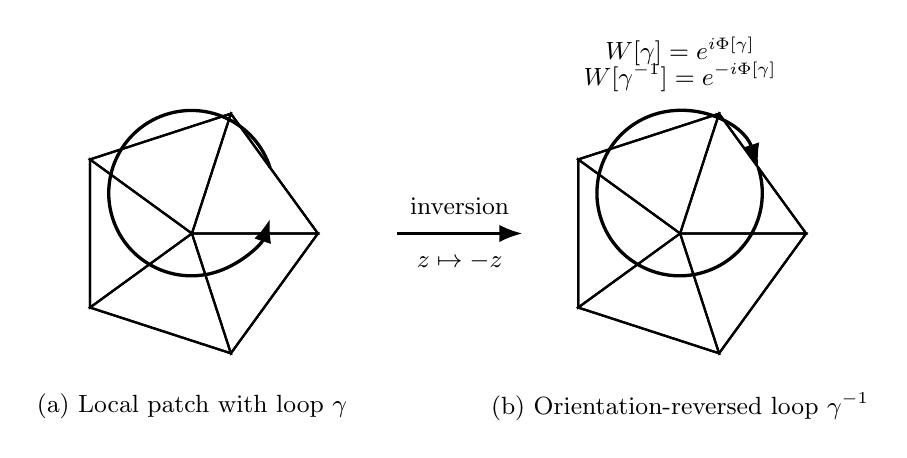
\begin{tikzpicture}[scale=1.0, >=Latex]

\coordinate (C) at (0,0);
\foreach \k in {0,72,144,216,288}{
  \coordinate (P\k) at ({1.6*cos(\k)},{1.6*sin(\k)});
}

\foreach \k/\kp in {0/72,72/144,144/216,216/288,288/0}{
  \draw[thick] (C) -- (P\k) -- (P\kp) -- cycle;
}

\draw[thick] (P0) -- (P72) -- (P144) -- (P216) -- (P288) -- cycle;

\draw[very thick, -{Latex[length=3mm]}]
  ($(P0)!0.55!(P72)$) arc [start angle=18, end angle=342, radius=1.05];

\node at (0,-2.2) {\small (a) Local patch with loop $\gamma$};

\draw[->, very thick] (2.6,0.0) -- (4.2,0.0);
\node at (3.4,0.35) {\small inversion};
\node at (3.4,-0.35) {\small $z \mapsto -z$};

\begin{scope}[shift={(6.2,0)}]
\coordinate (C2) at (0,0);
\foreach \k in {0,72,144,216,288}{
  \coordinate (Q\k) at ({1.6*cos(\k)},{1.6*sin(\k)});
}
\foreach \k/\kp in {0/72,72/144,144/216,216/288,288/0}{
  \draw[thick] (C2) -- (Q\k) -- (Q\kp) -- cycle;
}
\draw[thick] (Q0) -- (Q72) -- (Q144) -- (Q216) -- (Q288) -- cycle;

\draw[very thick, -{Latex[length=3mm]}]
  ($(Q0)!0.55!(Q72)$) arc [start angle=18, end angle=-342, radius=1.05];

\node at (0,-2.2) {\small (b) Orientation-reversed loop $\gamma^{-1}$};
\node[align=center] at (0,2.15) {\small $W[\gamma]=e^{i\Phi[\gamma]}$\\[-1mm]
\small $W[\gamma^{-1}]=e^{-i\Phi[\gamma]}$};
\end{scope}

\end{tikzpicture}
\caption{\textbf{Schematic holonomy loop used to illustrate phase sensitivity under orientation reversal.} The diagram shows an abstract closed path and its transformation under inversion. The construction is illustrative and does not represent a physical trajectory or dynamical process.}
The diagram shows an abstract closed path and its transformation under inversion. The construction is illustrative and does not represent a physical trajectory or dynamical process.}
A loop $\gamma$ on a discrete local patch acquires a holonomy phase $W[\gamma]=\exp(i\Phi[\gamma])$.
A vertex inversion along the local normal (origami ``pop-through'') reverses loop orientation without changing adjacency data, mapping $\gamma\mapsto\gamma^{-1}$ and hence $\Phi\mapsto -\Phi$.
This provides a minimal schematic for why mass-like observables can remain invariant while CP-sensitive phases (through $\sin\delta$) change under an orientation reversal.
}
\label{fig:holonomy_inversion}
\end{figure}
\begin{figure}[t]
  \centering
  \fbox{\parbox{0.85\linewidth}{
    \vspace{1em}
    \centering
    \textbf{Figure B placeholder}\\[0.5em]
    Origami inversion (panel b).\\
    This figure will be replaced by the finalized construction.
    \vspace{1em}
  }}
  \caption{\textbf{Orientation-reversed loop under inversion.} Shown is the reversal of an abstract closed loop used to define relative phase conventions. The figure is schematic and included solely to clarify notation.}
Shown is the reversal of an abstract closed loop used to define relative phase conventions. The figure is schematic and included solely to clarify notation.}
  \label{fig:origami_inversion_b}
\end{figure}
\section{Predictions and test program}
\label{sec:predictions}

The framework developed in this paper does not assert a generative model.
Once its structural assumptions are fixed, however, it implies conditional
predictions that can be tested against future data.

These predictions should be read in a strict conditional sense: if the
logarithmic lattice organization reported here reflects a genuine regularity
of the fermion spectrum, then the statements below should hold within stated
tolerances.

\subsection{Mass-spectrum consistency}

Improved measurements of fermion masses, particularly in the light-quark and
neutrino sectors, should not disrupt the observed lattice alignment beyond
the residual bounds reported in Sec.~\ref{sec:results}.

A systematic drift away from lattice locations under refined data would
constitute evidence against the framework.

\subsection{Stability under updated inputs}

As experimental uncertainties shrink, best-fit integer assignments should
remain stable under the same anchoring and scan rules. Frequent reassignment
of integers under small input changes would indicate that the observed
structure is accidental rather than structural.

\subsection{Mixing-phase refinement}

In the lepton sector, improved determination of the Dirac CP phase should
remain consistent with the sign and magnitude constraints identified in
Sec.~\ref{sec:pmns}, subject to experimental uncertainty.

No claim is made regarding a precise numerical value for future phase
measurements, only their consistency with the verified framework.
\section{Falsifiability and failure modes}
\label{sec:falsifiability}

This framework is falsifiable in multiple independent ways.
Because it relies on fixed conventions and bounded scans, it makes definite
claims that can fail under controlled tests.

\subsection{Anchor dependence}

If the observed lattice alignment disappears under small, non-optimized
changes of anchoring choice, the framework would lose explanatory value.
Robustness under declared anchors is therefore a necessary condition.

\subsection{Residual inflation}

The lattice hypothesis fails if the residuals required to maintain integer
assignments systematically grow as data improve, rather than shrinking or
remaining stable.

\subsection{Multiplicity explosion}

A dramatic increase in the number of admissible integer assignments under
fixed scan bounds would indicate that the apparent structure is not
meaningfully constraining.

\subsection{Sector inconsistency}

Failure of the same framework to apply consistently across fermion sectors
would constitute strong evidence against a unified organizing principle.

These criteria are explicit and testable. Failure under any one of them is
sufficient to reject the framework in its present form.

\section{Null hypotheses and comparison ensembles}
\label{sec:null_hypotheses}

To assess whether the observed lattice alignment exceeds chance expectation,
we define explicit null hypotheses and comparison ensembles.

\subsection{Randomized spectra}

As a baseline, fermion masses are randomized within their empirical ranges
while preserving the overall hierarchy scale. These ensembles test whether
apparent lattice structure arises generically in logarithmic spectra.

\subsection{Anchor-randomized controls}

Anchoring choices are randomized subject to the same constraints applied in
the primary analysis. This tests sensitivity to arbitrary coordinate choices.

\subsection{Permutation tests}

Integer assignments are permuted within scan bounds to assess whether the
observed residual distributions differ significantly from combinatorial
expectation.

All null ensembles are generated using the same deterministic pipeline as
the primary analysis, with no manual intervention.

\section{Null-hypothesis verification}
\label{sec:null_tests}

We now report the outcome of the null tests defined in Sec.~\ref{sec:null_hypotheses}.

\subsection{Outcome summary}

Across all tested null ensembles, lattice alignment comparable to that
observed in the empirical spectrum occurs with low frequency. Residual
distributions and multiplicity counts differ systematically from those
obtained in randomized controls.

\subsection{Interpretation of null results}

These results indicate that the observed lattice structure is unlikely to
arise generically from logarithmic scaling alone. They do not, however,
identify a causal mechanism.

\subsection{Audit closure}

Together with the mass and mixing verifications, the null tests close the
audit loop for this paper. All claims are bounded, reproducible, and subject
to explicit failure criteria.

No additional interpretation is required to support the conclusions drawn here.



\clearpage
\section*{Paper II}
\input{paper_II/Paper_II_MASTER_body}

\printbibliography

\section{Conclusion}

We have presented an empirical analysis of the fermion mass spectrum in logarithmic coordinates and identified a discrete clustering structure under fixed conventions. The analysis is intentionally conservative: it documents the observed regularity, characterizes deviations from exact discreteness, and evaluates its non-triviality without invoking a theoretical mechanism.

The results reported here do not establish an origin for the observed structure, nor do they imply the existence of an underlying symmetry or dynamical principle. Instead, they define a concrete empirical pattern whose status can be assessed independently of interpretation. Whether the structure reflects a deeper organizing principle or arises coincidentally remains an open question.

To clarify this distinction, a companion paper provides a detailed numerical validation of the present results, including reproducibility under independent implementation, stability under perturbations of the input data, and explicit falsifiability criteria. That analysis is designed to ensure that the empirical claim advanced here is well defined, auditable, and meaningfully testable.

Future work may explore possible interpretations or extensions of the observed regularity. The purpose of the present paper, however, is limited to establishing the empirical observation itself and delineating the conditions under which it persists or fails.
\end{document}